\section{Recommendation system design}

\noindent Recommendation systems in e-commerce platforms leverage user data and machine learning algorithms to provide personalized product suggestions. They enhance user experience, increase customer engagement facilitate product discovery, optimize inventory management, and personalize marketing campaigns.

\subsection{Recommendation system process}

\noindent To build an effective personalized architecture, it is crucial to integrate offline and online components seamlessly. A compromise approach is nearline computation, which combines the data processing capabilities of offline systems with real-time responsiveness to serve users effectively. This integration allows for efficient calculations and processing of data offline while still providing immediate responses and services to users online.

\begin{itemize}
    \item Offline computation takes place for batch processing, in which huge data manipulation and algorithm complexity will give priority over than response time requirements. This is where data will be mainly stored and handled since offline computation empowers for applying different algorithms for comparison and allowing a less limitations on amount of data to be processed
    \item Online computation, on the other hand, offers a great response time on real-time users events which helps the system deliver a better experience for customers. Furthermore, it adapts availability and Service Level Agreements (SLAs) which states the maximum latency for a request from clients while waiting for the recommendation to appear. 
     \item Nearline computation is a compromise solution since it can serve results with a response time of online method, along with compute large amount of data using complex algorithm and store it for later use as offline method. 
\end{itemize}

\begin{figure}[H]
    \centering
    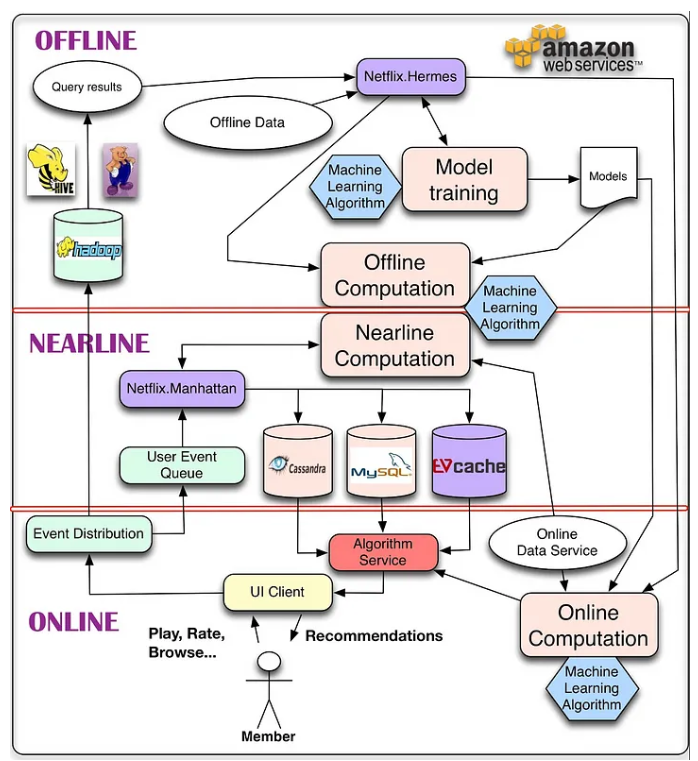
\includegraphics[width=0.7\linewidth]{image/Architecture/netflix.png}
    \caption{Netflix overall system diagram}
    \label{fig:enter-label}
\end{figure}

\noindent Combining all three methods is vital for creating a highly potent recommendation system as they mutually complement each other. But how can we realize this complex system architecture if we have insufficient resources?

\subsection{Gorse to the rescue}

\noindent Gorse, an open-source recommender engine, offers several advantages. It provides rich documentation, making it easier for developers to understand and utilize its features. The API is user-friendly, and it also offers support for a client library in Java, enabling seamless integration into Java-based projects. Compared to other open-source recommender engines, Gorse requires minimal development effort, making it a time-efficient choice. However, Gorse does have some limitations. One area where it falls short is in terms of expressive power in representing user-item interactions. This means that it may not capture complex patterns or relationships between users and items as effectively as some other recommender engines.

\begin{figure}[H]
    \centering
    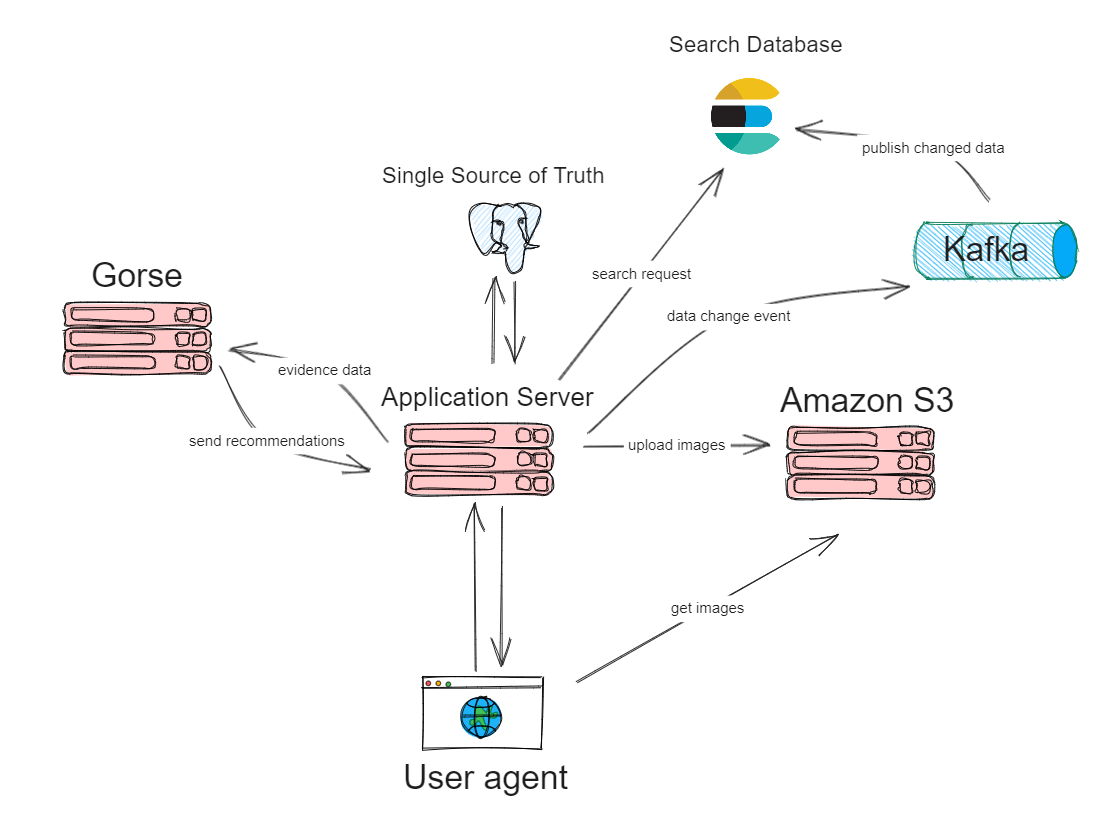
\includegraphics[width=1\linewidth]{image/Architecture/high-level.png}
    \caption{High-level View of Architecture}
    \label{fig:enter-label}
\end{figure}

\noindent As the diagram depiction, Gorse plays an important role in the system in which evidence transmission, data computational process, and recommendations response will be abstracted into handy APIs for developers. \\

\noindent Another aforementioned area that has also been taken into account is that how users data and computed data can be stored and synchronized in the application.\\ 
The overall architecture will have a single source of truth for all the data. That makes use of PostgreSQL database. Meanwhile, our system also includes another data store whose sole purpose is to effectively retrieve information. The use of two databases exposes the system to data inconsistency problems. Therefore, we need an architectural solution to resolve the issue


\subsubsection{Capturing Data Changes (CDC)}

\begin{figure}[H]
    \centering
    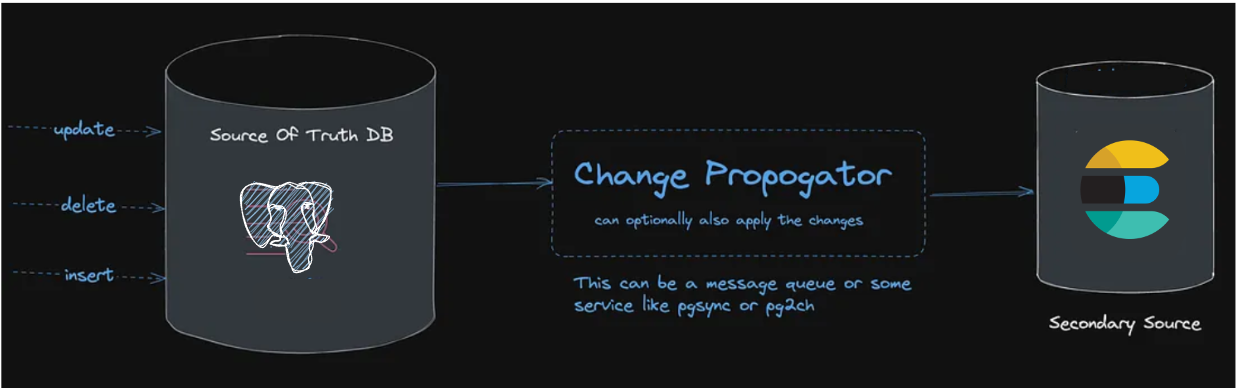
\includegraphics[width=1\linewidth]{image/Architecture/cdc.png}
    \caption{Capturing Data Changes Illustration}
    \label{fig:enter-label}
\end{figure}

 A software process that detects and monitors data modifications within a database. It enables the seamless movement and processing of data in real-time or near-real-time, ensuring that new database events are promptly captured and processed.

\subsubsection{Message broker (event-driven approach)}

\begin{figure}[H]
    \centering
    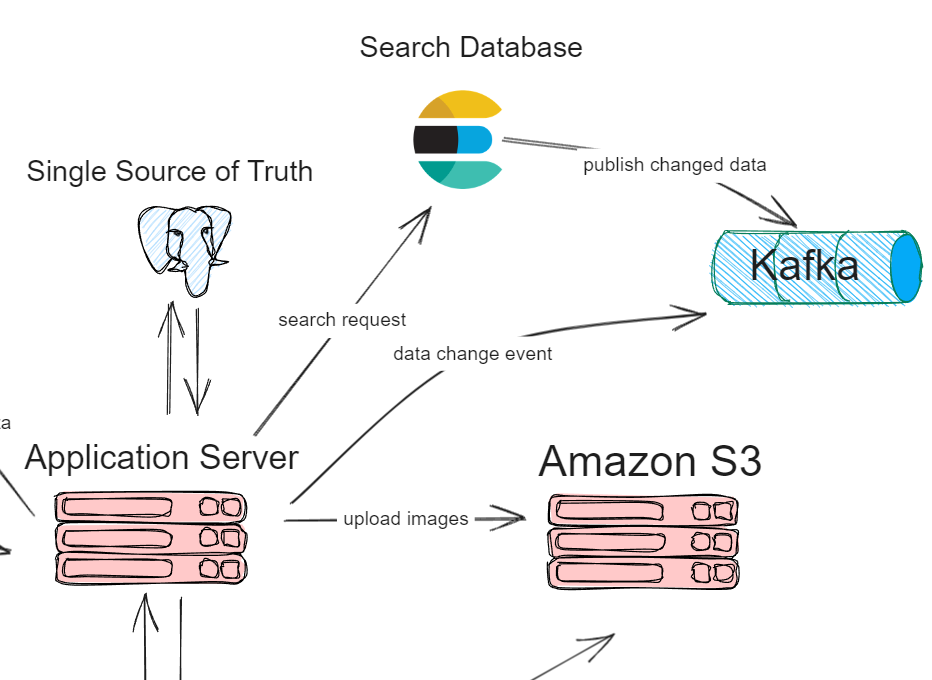
\includegraphics[width=0.7\linewidth]{image/Architecture/kafka.png}
    \caption{Message broker - Kafka}
    \label{fig:enter-label}
\end{figure}

\noindent The application server is responsible for the single source of truth. Any write/update/delete operations that lead to data changes must be carried out by the back-end application. After updating the data state in the primary source, it must send an event to a message broker, Kafka in our architecture, such that the data changes will notify the Elasticsearch database. \\ \\
The system’s objective is to implement the main functions that we intend to improve for an e-commerce website, and other add-in features for an e-commerce system are omitted for the sake of simplicity. One of them is the subsytem for e-commerce data analysis that requires to use of another data store solution to implement online analytical processing (OLAP) functions. If we go for CDC solution, it means that we compensate for future changes. To add a third data store to the system, we must either implement CDC for the new one or migrate the whole architecture to use a message broker. Therefore, our team decided to go for event-driven architecture to decrease the foreseeable cost although it requires more overhead cost for the broker.\\

\subsection{Evidence collecting}
\noindent Evidence is any interaction that the system collects via customer interaction with the system. The collecting process can be categorized as \textbf{implicit} or \textbf{explicit}.

\subsubsection{Implicit evidence}
\begin{itemize}
    \item User rating on the purchased products
    \item User comments on the purchased products
\end{itemize}

\subsubsection{Explicit evidence}
\begin{itemize}
    \item \textbf{Page View}
    \item \textbf{Page Duration:} the longer users stop browsing and investigate an item, the more interested they are
    \item \textbf{Expansion clicks:} After a read on a brief overview of the item description, the user still wants to delve further to gain deeper knowledge about the product, which proves the attraction of the item toward the user. 
    \begin{figure}[H]
    \centering
    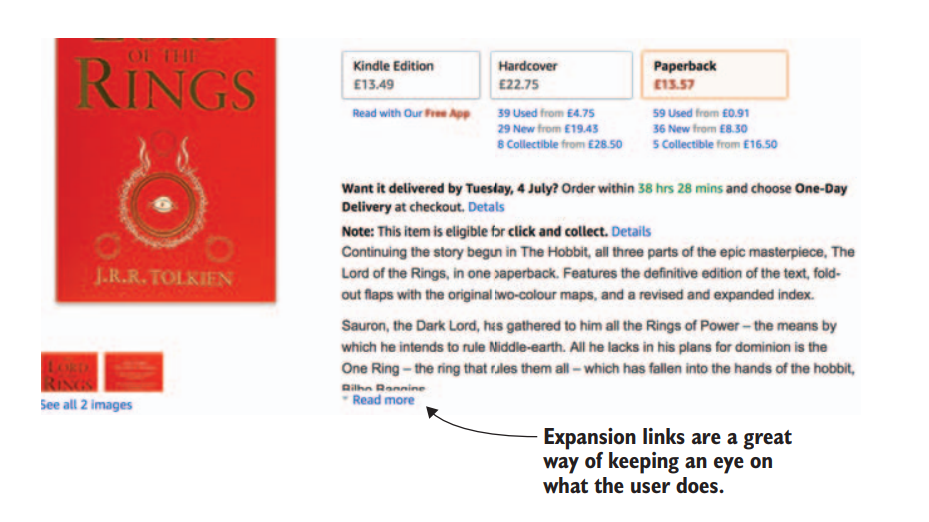
\includegraphics[width=1\linewidth]{image/Architecture/expansion links.png}
    \caption{Expansion Click Illustration}
    \label{fig:enter-label}
\end{figure}
    \item \textbf{Scroll down in product detail page:} more comparison-rich information related to a product is often included by the e-commerce website at the near end of the product detail page. After getting knowledge about the product to consider if it is the right thing to buy, the user will keep going to the next phase of conversion in which they start comparing different products of the same line or seeking to social comments to make the final decision. The act of rolling to that section absolutely presents their interest in the current item.
    \item \textbf{Add a product to the wishlist:} the act implies that the user will likely buy the item on a future visit.
    \item \textbf{Search terms:} this is also a good source to help Recommender deduce the products that the searcher is currently keen on and hence make the immediate changes in the recommendation.
    \item \textbf{Purchase a product:} Purchase history to learn about the interest of a user and recommend a similar item the next time
    \item \textbf{User sharing}
\end{itemize}

\subsection{Application of recommendation in BKTechStore}
\begin{itemize}
    \item Give the user the most relevant recommendations to their need by filtering the shown-up catalog. Because the website’s purpose is not to keep the user at the website as long as possible but to aid the customer in seeking products that meet their need and increase user experience as a result.
    \item Suggest related items that user may interest in the checkout process (item-based recommendation)
\end{itemize}